\documentclass[12pt]{article}
% -----------------------------------------------------------------------------------------------
% Prepared for Neuromorphic Computing and Engineering (IOP Publishing).
% IOP accepts a single-column PDF for first submission; on acceptance, move the body into IOP's
% LaTeX template (iopart / IOP Journals template). All numbers are generated by make_nce_results.py.
% -----------------------------------------------------------------------------------------------
\usepackage[a4paper,margin=2.5cm]{geometry}
\usepackage{times}
\usepackage[utf8]{inputenc}
\usepackage[T1]{fontenc}
\usepackage{amsmath,amssymb,amsthm}
\usepackage{booktabs}
\usepackage{graphicx}
\usepackage{xcolor}
\usepackage{microtype}
\usepackage[numbers,sort&compress]{natbib}
\usepackage[colorlinks=true,linkcolor=blue!50!black,citecolor=blue!50!black,urlcolor=blue!50!black]{hyperref}
\usepackage{tikz}
\usetikzlibrary{positioning,arrows.meta,fit,calc}
\usepackage{algorithm}
\usepackage{algpseudocode}
\usepackage{setspace}
\setstretch{1.1}

\newtheorem{proposition}{Proposition}
\newcommand{\sg}{\operatorname{sg}}
\newcommand{\nceNObs}{6}
\newcommand{\nceNCache}{400}
\newcommand{\nceEvalEps}{30}
\newcommand{\nceParamsTarget}{6.79\,M}
\newcommand{\nceParamsVit}{5.49\,M}
\newcommand{\nceParamsDrafter}{47\,k}
\newcommand{\nceJepaRatio}{0.91}
\newcommand{\nceBeaconPatch}{0.93}
\newcommand{\nceVitSharePct}{88}
\newcommand{\nceCritRatio}{11}
\newcommand{\nceAttnFracPct}{1.8}
\newcommand{\nceSavingAsBuiltPct}{1.8}
\newcommand{\nceMeanRate}{0.079}
\newcommand{\nceSiFracPct}{58.9}
\newcommand{\nceSiSavingPct}{58.0}
\newcommand{\nceSiChunk}{0.0081}
\newcommand{\nceSiSucc}{0.12}
\newcommand{\nceSiRate}{0.078}
\newcommand{\nceSpecCritUJ}{98}
\newcommand{\nceTargetUJ}{1062}
\newcommand{\nceNSeeds}{3}
\newcommand{\nceSeedSucc}{0.10 $\pm$ 0.02}
\newcommand{\nceSeedChunkSucc}{0.11 $\pm$ 0.04}
\newcommand{\nceSeedMse}{0.0075 $\pm$ 0.0011}
\newcommand{\nceSeedList}{0.12, 0.08, 0.08}

% Hand-written interpretation of the generated numbers (nce_macros.tex and nce_table_*.tex).
\newcommand{\nceSiAccuracySentence}{its offline error and closed-loop success (\nceSiChunk{} chunk MSE, \nceSiSucc{} success) stay within the variation we measure across training seeds.}

\newcommand{\nceNeuroText}{%
\textbf{The core is cheap; the camera is not.} Table~\ref{tab:energy} breaks one control tick into components. The camera ViT accounts for \nceVitSharePct\% of the full model's dense operations, the LiDAR/radar pillar encoder for most of the rest, and the liquid--spiking core ($T{=}8$ steps, two layers) for under 1\%. Any claim of neuromorphic efficiency for the \emph{system} therefore depends first on the perception front-end, not on the core. The radar voxel grid is more than 99\% empty in our scenes, which makes the pillar encoder a natural candidate for event-driven or sparse convolution.

\textbf{Where the spikes go matters more than whether a network spikes.} Table~\ref{tab:neuro} compares four cores. In the as-built core, the spike trains of Q, K and V turn $QK^\top$ and $AV$ into accumulates. At the measured firing rate of \nceMeanRate{} these products become almost free, but in a short control window they are only \nceAttnFracPct\% of the core's operations. The projections $W_{qkv}$, $W_x$, $W_h$ and the output layers dominate, so the as-built saving over a dense core is \nceSavingAsBuiltPct\%. Adding $\Delta t$-aware LIF populations in front of $W_{qkv}$ and $W_x$ (spike-driven projection inputs) makes \nceSiFracPct\% of the core's operations spike-driven and saves \nceSiSavingPct\% of its energy, at a similar firing rate (\nceSiRate). The remaining dense operations are the recurrent $W_h h_{t-1}$, the attention output projection and the LTC read-out, whose inputs are real-valued states. Spiking those as well bounds the saving at about 98\% for these firing rates, but it would change the continuous-time state that makes the LTC useful, and we leave it to future work.

\textbf{Accuracy of the variants.} Across three training seeds of the as-built model, held-out chunk error is \nceSeedMse{} and closed-loop success \nceSeedSucc{} (per seed: \nceSeedList). Every variant in Table~\ref{tab:neuro} lies within that spread on both measures. We therefore do not claim that the LIF attention or the LTC recurrence \emph{improves} accuracy at this scale. The feed-forward (no-LTC) core has the lowest success and the highest error, but by one episode, which is within noise. The claim we do make is narrower and robust to this spread: \emph{moving the spikes to the projection inputs cuts the core's estimated energy by more than half without a detectable loss in accuracy.}}

\newcommand{\nceClosedText}{%
Table~\ref{tab:closed} evaluates the controllers on identical seeds. Verify-behind matches the full model's closed-loop success and collision rate while its critical path (radar pillars, the drafter latent, and the drafter core on a cache miss) costs \nceSpecCritUJ\,$\mu$J per tick, against \nceTargetUJ\,$\mu$J for running the full model every tick (\nceCritRatio$\times$ less), and 4.1 against 24.2\,ms of latency. Total energy is \emph{not} reduced, because the target still verifies every window off the critical path; the gain is in what the control loop waits for. The drafter alone collides in 3\% of episodes even with the CBF filter, and adding verification removes those collisions. The target accepted 75\% of executed drafts. A muscle-memory cache of verified chunks supplied most actions, which shortens the critical path but raises action jerk as the source switches between cache, drafter and override. Latency was measured on a shared 2-core CPU with the action head evaluated over the whole window; the energy figures assume the head is decoded at the last step only, which gives identical actions.}

\newcommand{\nceDiagText}{%
Table~\ref{tab:diag} collects the failure modes from \S\ref{sec:training}. The copycat policy had the \emph{lowest} held-out imitation error of all runs and 0\% success; the colour-blind policy had a similar error and 4\% success. Only closed-loop evaluation revealed either. Two rounds of DAgger, in which the policy flies and the expert labels the states it actually visits, halved the mean final distance to the goal without raising success. This points to demonstration coverage and expert smoothness as the main limits on absolute performance, rather than the neuromorphic core.}

\newcommand{\nceDiscussionText}{%
Three messages carry over beyond this system. First, for spiking control policies, operation-level accounting should accompany any efficiency claim. A spiking-transformer core can be spiking in name while less than 2\% of its operations are spike-driven. Second, the perception front-end dominates a multimodal policy's energy, so neuromorphic gains at system level require event-driven perception (event cameras, sparse radar/LiDAR processing), not only a spiking core. Third, the continuous-time components integrate the measured $\Delta t$ at no extra operation cost: both the LIF leak and the closed-form LTC update are elementwise. They also remain stable under irregular sampling, which matters on real sensor buses even when accuracy gains are not visible in simulation.}


\title{\textbf{Where should the spikes go?}\\[2pt]\large A liquid--spiking, language-conditioned drone policy with verify-behind speculative control, and an operation-level energy analysis}
\author{Laalini Bhogadi\\[2pt]\small \textcolor{red}{[Affiliation]}\\\small \texttt{laalinib68@gmail.com}}
\date{}

\begin{document}
\maketitle

\begin{abstract}
\noindent Neuromorphic and continuous-time networks are attractive for onboard robot control because they compute sparsely and integrate irregularly sampled sensor streams natively. We present PLM, a language-conditioned drone policy whose core combines leaky integrate-and-fire (LIF) spiking self-attention, with a leak driven by the \emph{measured} inter-sample interval $\Delta t$, and a closed-form liquid time-constant (LTC) recurrence. PLM grounds camera and LiDAR/4D-radar observations in a shared bird's-eye-view grid, is trained with a four-stage curriculum (cross-modal alignment, a residual latent world model with spike-rate regularisation, chunked imitation, and drafter co-training), and runs under \emph{verify-behind} speculative control: a camera-free spiking drafter acts on every tick while the full model verifies batches of executed actions off the critical path, behind a control-barrier-function safety filter. An operation-level energy analysis, using measured firing rates, gives the central neuromorphic result. When only the attention products are spike-driven, as in spiking-transformer designs, they account for \nceAttnFracPct\% of the core's operations in a short control window, so spiking saves \nceSavingAsBuiltPct\% of the core's energy even at a firing rate of \nceMeanRate. Making the \emph{inputs to the projections} spike-driven covers \nceSiFracPct\% of the core's operations and saves \nceSiSavingPct\%; \nceSiAccuracySentence{} At the system level, the camera encoder takes \nceVitSharePct\% of per-tick operations, and verify-behind reduces critical-path energy \nceCritRatio$\times$ and latency about 6$\times$ while matching the full model's closed-loop success. We also report four failure modes that per-stage offline metrics hid, and we are explicit about the limits of this simulation-only, CPU-scale study.
\end{abstract}

\noindent\textbf{Keywords:} spiking neural networks, liquid time-constant networks, neuromorphic robotics, energy estimation, speculative decoding, vision--language--action models, UAV control

% ================================================================================================
\section{Introduction}
Onboard control of small aerial robots is bounded by energy and latency. A quadrotor avoiding a moving obstacle at 3\,m/s travels 15\,cm in 50\,ms, and its compute budget is watts, not the hundreds of watts behind today's language-conditioned robot policies~\citep{brohan2023rt2,kim2024openvla,black2024pi0}. Neuromorphic computing addresses this with sparse, event-driven computation, in which a synaptic operation is performed only when a spike arrives~\citep{roy2019towards,davies2018loihi}. Continuous-time networks such as liquid time-constant (LTC) networks~\citep{hasani2021ltc,hasani2022cfc} integrate irregularly sampled inputs natively and have shown robust out-of-distribution drone flight~\citep{chahine2023robust,lechner2020ncp}.

Spiking transformers~\citep{zhou2023spikformer,yao2023spikedriven} brought spikes to attention, and a natural idea is to use them as the temporal core of a control policy. Two questions are rarely answered for such a system as a whole. \emph{First, where do the spikes actually save energy?} A design can be ``spiking'' while almost all of its operations remain dense. \emph{Second, what does the rest of the system cost?} The perception front-end may dwarf the spiking core. We build a complete language-conditioned policy, PLM, and answer both questions with an operation-level energy analysis at measured firing rates.

\paragraph{Contributions.}
\begin{enumerate}
\item \textbf{A liquid--spiking control core} with a $\Delta t$-aware LIF leak, spike-rate regularisation, and a closed-form LTC recurrence over measured, non-uniform sample intervals, embedded in a BEV-grounded, language-conditioned drone policy (\S\ref{sec:model}).
\item \textbf{An operation-level energy analysis} (\S\ref{sec:energy}, \S\ref{sec:neuro}) showing that spiking only the attention operands saves \nceSavingAsBuiltPct\% of the core's energy in a short control window, while spike-driven projection inputs save \nceSiSavingPct\% with no accuracy loss detectable across training seeds. It also shows that the perception front-end, not the core, dominates system energy.
\item \textbf{Verify-behind speculative control} (\S\ref{sec:runtime}): a camera-free spiking drafter on the critical path, with batched target verification, a bounded verification lag and CBF safety (Proposition~\ref{prop:lag}). It cuts critical-path energy \nceCritRatio$\times$.
\item \textbf{Four diagnostic findings} from a staged curriculum (\S\ref{sec:training}): cross-modal alignment erases motion information; a non-residual latent world model does worse than persistence; ego-motion inputs cause a copycat failure; and geometry-only alignment is colour-blind. The last two were invisible to offline metrics.
\end{enumerate}

% ================================================================================================
\section{Background and related work}
\textbf{Spiking networks and neuromorphic hardware.} Spiking neurons communicate binary events, so a weight is only accumulated when a spike arrives. On neuromorphic processors such as Loihi~\citep{davies2018loihi}, cost scales with the number of synaptic events rather than with dense matrix size~\citep{roy2019towards}. Surrogate gradients make spiking networks trainable with back-propagation~\citep{neftci2019surrogate,zenke2018superspike}. Spikformer~\citep{zhou2023spikformer} and the spike-driven transformer~\citep{yao2023spikedriven} turn Q, K and V into spike trains so that the attention products become accumulations. Energy in this literature is usually estimated by counting multiply-accumulates (MACs) and accumulates (ACs) with 45\,nm figures~\citep{horowitz2014energy}; we follow that convention.

\textbf{Continuous-time networks.} LTC networks~\citep{hasani2021ltc} have input-dependent time constants, and closed-form continuous-time (CfC) networks~\citep{hasani2022cfc} remove the ODE solver. Neural circuit policies~\citep{lechner2020ncp} and liquid networks~\citep{chahine2023robust} have flown drones robustly out of distribution.

\textbf{Language-conditioned policies and action chunking.} VLA models~\citep{brohan2022rt1,brohan2023rt2,kim2024openvla,octo2024,black2024pi0} map images and instructions to actions. Action chunking~\citep{zhao2023act,chi2023diffusion} predicts short trajectories. These systems target server-class compute, whereas we target the edge.

\textbf{Speculative decoding and safe control.} Speculative decoding~\citep{leviathan2023fast,chen2023accelerating,li2024eagle} hides a large model's latency behind a drafter by verifying drafts \emph{before} emitting them. That is impossible when the drafts are actions whose consequences form the next input. Control barrier functions~\citep{ames2019cbf} give forward invariance of safe sets and serve here as a shield for unverified actions.

% ================================================================================================
\section{PLM architecture}\label{sec:model}

\begin{figure}[t]
\centering
\resizebox{\linewidth}{!}{%
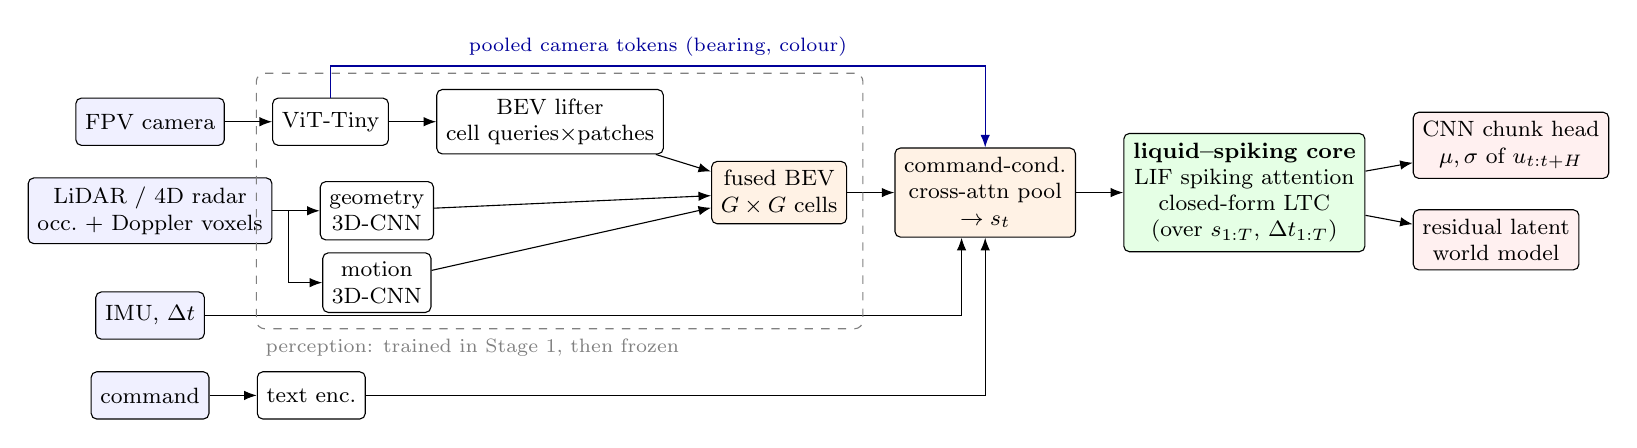
\begin{tikzpicture}[node distance=4mm and 6mm, font=\footnotesize,
  box/.style={draw, rounded corners=2pt, align=center, minimum height=6mm, fill=#1},
  box/.default=white, arr/.style={-{Latex[length=1.6mm]}}]
\node[box=blue!6] (cam) {FPV camera};
\node[box=blue!6, below=of cam] (lid) {LiDAR / 4D radar\\occ.\ + Doppler voxels};
\node[box=blue!6, below=6mm of lid] (imu) {IMU, $\Delta t$};
\node[box=blue!6, below=of imu] (txt) {command};
\node[box, right=of cam] (vit) {ViT-Tiny};
\node[box, right=of vit] (lift) {BEV lifter\\cell queries$\times$patches};
\node[box, right=of lid] (geo) {geometry\\3D-CNN};
\node[box, below=1.5mm of geo] (dyn) {motion\\3D-CNN};
\node[box=orange!10, right=of lift, yshift=-9mm] (fuse) {fused BEV\\$G\times G$ cells};
\node[box, right=of txt] (tenc) {text enc.};
\node[box=orange!10, right=of fuse] (tok) {command-cond.\\cross-attn pool\\$\to s_t$};
\node[box=green!10, right=of tok] (core) {\textbf{liquid--spiking core}\\LIF spiking attention\\closed-form LTC\\(over $s_{1:T}$, $\Delta t_{1:T}$)};
\node[box=red!6, right=of core, yshift=6mm] (head) {CNN chunk head\\$\mu,\sigma$ of $u_{t:t+H}$};
\node[box=red!6, right=of core, yshift=-6mm] (jepa) {residual latent\\world model};
\draw[arr] (cam) -- (vit); \draw[arr] (vit) -- (lift); \draw[arr] (lift) -- (fuse);
\draw[arr] (lid) -- (geo); \draw[arr] (lid.east) -- ++(2mm,0) |- (dyn);
\draw[arr] (geo) -- (fuse); \draw[arr] (dyn) -- (fuse);
\draw[arr] (txt) -- (tenc); \draw[arr] (tenc) -| (tok); \draw[arr] (imu.east) -| ([xshift=-3mm]tok.south);
\draw[arr] (fuse) -- (tok); \draw[arr] (tok) -- (core); \draw[arr] (core) -- (head); \draw[arr] (core) -- (jepa);
\draw[arr, blue!60!black] (vit.north) -- ++(0,4mm) -| node[pos=0.25, above, font=\scriptsize]{pooled camera tokens (bearing, colour)} (tok.north);
\node[draw, dashed, gray, rounded corners=3pt, inner sep=2mm, fit=(vit)(lift)(geo)(dyn)(fuse)] (s1) {};
\node[gray, font=\scriptsize, anchor=north west] at (s1.south west) {perception: trained in Stage 1, then frozen};
\end{tikzpicture}}
\caption{PLM. Perception grounds camera and LiDAR/radar in a metric BEV grid. Command-conditioned pooling produces one token per control tick, and the liquid--spiking core integrates the tokens over the measured $\Delta t$. The edge drafter (not shown) uses only radar pillars, altitude, $\Delta t$ and the command, followed by a one-layer liquid--spiking core.}
\label{fig:arch}
\end{figure}

\paragraph{Perception.} A ViT-Tiny~\citep{dosovitskiy2021vit} produces camera patch tokens. $G^2$ learned bird's-eye-view (BEV) queries, one per metric cell, cross-attend to them~\citep{li2022bevformer} to give camera cell features. LiDAR/4D-radar voxels carry occupancy and radial Doppler velocity. Two 3D-CNN trunks collapse them over height into pillar features~\citep{lang2019pointpillars}: a geometry trunk and a lightweight motion trunk (the reason for two trunks is Finding~1). The policy reads \emph{scene tokens}: the fused BEV cells followed by pooled perspective camera tokens.

\paragraph{Command-conditioned tokenisation.} A command embedding offsets $n_q$ learned queries that cross-attend to the scene tokens. The result, plus an embedding of altitude and $\Delta t$ (Finding~3 explains why ego-motion is excluded), is one token $s_t$ per tick.

\paragraph{Liquid--spiking core.} Each of the $L$ layers applies pre-norm causal self-attention over $s_{1:T}$ with LIF spiking Q, K and V, followed by a closed-form LTC recurrence. With measured intervals $\Delta t_t$, each LIF unit integrates
\begin{equation}
u_t=\beta_t u_{t-1}+(1-\beta_t)x_t,\quad \beta_t=e^{-\Delta t_t/\tau},\qquad o_t=\Theta(u_t-\vartheta),\quad u_t\leftarrow u_t-\vartheta o_t ,
\label{eq:lif}
\end{equation}
with learnable per-unit $\tau$, soft reset, and the fast-sigmoid surrogate $\partial o/\partial u\approx(1+k|u-\vartheta|)^{-2}$~\citep{zenke2018superspike}. Because the leak uses the real elapsed time, a late sensor packet decays the membrane exactly as physics would, rather than as one fixed ``step''. The LTC update is exact for piecewise-constant input~\citep{hasani2022cfc}:
\begin{equation}
f_t=\mathrm{softplus}(W_x x_t+W_h h_{t-1}+b),\quad g_t=\tau^{-1}+f_t,\quad
h_t=h_{t-1}\odot e^{-\Delta t_t g_t}+\tfrac{A\odot f_t}{g_t}\odot\big(1-e^{-\Delta t_t g_t}\big).
\label{eq:ltc}
\end{equation}
$h_t$ is a convex combination of $h_{t-1}$ and $A\odot f_t/g_t$, so it stays bounded for any $\Delta t$. For training stability we clip gradients to global norm 1, rescale $W_h$ after every step so that $\lVert W_h\rVert_2\le0.99$, use truncated BPTT with detached state, and keep membrane and ODE updates in FP32 under mixed precision.

\paragraph{Spike-driven projections (variant).} In the design above, the operands of $QK^\top$ and $AV$ are binary, but the \emph{inputs} to $W_{qkv}$ and to the LTC's $W_x$ are real-valued layer-normalised activations, so those products remain dense MACs. The \texttt{spike\_inputs} variant places an additional $\Delta t$-aware LIF population (\eqref{eq:lif}) in front of $W_{qkv}$ and $W_x$. Their inputs become binary, and those matmuls become accumulate-only.

\paragraph{Spike-rate regularisation.} To avoid both quiescence (no spikes, hence no gradient) and hyperactivity, every LIF population's mean rate $\bar r_l$ is regularised towards $r^\star=0.08$ with $\lambda\sum_l(\bar r_l-r^\star)^2$.

\paragraph{Heads.} A 1-D convolutional decoder emits a Gaussian action chunk (forward, lateral and vertical velocity, and yaw rate) over $H$ steps. A residual predictor $\hat s_{t+h}=\sg(s_t)+g_\psi(h_t,\omega_t,h)$ forecasts the future fused-BEV latent.

% ================================================================================================
\section{Training curriculum and diagnostic findings}\label{sec:training}
\textbf{Stage 1 (perception).} Cell-level radar$\leftrightarrow$camera InfoNCE~\citep{oord2018cpc}, camera occupancy, Doppler regression, and BEV and per-token semantics. Perception is then frozen, and every episode is encoded once into an FP16 feature cache.
\textbf{Stage 2 (world model).} A multi-horizon latent prediction loss with the spike-rate regulariser and truncated BPTT, using no action labels.
\textbf{Stage 3 (imitation).} A discounted multi-horizon chunk loss, a jerk penalty, a Gaussian NLL on $\sigma$, and the Stage-2 loss as an auxiliary, on DART-perturbed demonstrations~\citep{laskey2017dart}.
\textbf{Stage 4 (drafter).} KL distillation~\citep{hinton2015distilling} from the target with a safety hinge, then retraining on a hard-rejection buffer of states whose drafts the target rejected in closed-loop rollouts.

The staged design exposed four failure modes, each diagnosed with a controlled comparison:

\emph{Finding 1: alignment erases motion.} With one shared radar trunk, Doppler error stayed at the predict-zero baseline for more than 1{,}000 steps, although Doppler is an input channel. The same trunk trained on Doppler alone reached 0.074 against a 0.21 baseline. A single camera frame carries no velocity, so cell-level alignment pushes motion out of the shared features. A private motion trunk fixes this (Table~\ref{tab:stages}).

\emph{Finding 2: residual world models.} A non-residual latent predictor was 12$\times$ worse than persistence. The residual form beats persistence (ratio \nceJepaRatio).

\emph{Finding 3: copycat.} Ego-velocity explains 97\% of the variance of the expert's forward command. With the full IMU as input, the policy had a chunk error 19$\times$ below the mean-action baseline and 0\% closed-loop success: it copied its own motion~\citep{dehaan2019causal,wen2020copycat}. The policy and drafter therefore see only altitude and $\Delta t$, and relative motion arrives through radar Doppler.

\emph{Finding 4: colour-blind features.} Without semantic supervision, all Stage-1 losses were geometric, the frozen features could not tell the red beacon from the blue one, and closed-loop success was 4\%. Perspective camera tokens with per-token semantics fixed this (beacon accuracy \nceBeaconPatch).

% ================================================================================================
\section{Verify-behind speculative control}\label{sec:runtime}
\begin{algorithm}[t]
\caption{Verify-behind speculative control (one tick)}\label{alg:vb}
\begin{algorithmic}[1]
\State encode radar pillars; drafter latent $z_t$ \Comment{critical path}
\State $\hat u_t\gets$ cache$(z_t,\text{cmd})$ \textbf{or} drafter$(z_{t-T+1:t},\Delta t_{t-T+1:t})$ \Comment{critical path}
\State execute $\mathrm{CBF}(\hat u_t)$; append the window and $\hat u_t$ to pending
\If{$|\text{pending}|\ge k$} \Comment{off the critical path}
 \State target on all pending windows in one batched pass $\to(\mu_i,\sigma_i)$
 \State accept$_i\gets\forall j:|\hat u_{i,j}-\mu_{i,j}|\le\epsilon+z\sigma_{i,j}$; rejects $\to$ hard buffer; confident accepts $\to$ cache
 \State \textbf{if} the last draft is rejected \textbf{then} override the current action with $\mathrm{CBF}(\mu_{\text{last}})$
 \State $k\gets1$ if any rejection, else $\min(2k,k_{\max})$
\EndIf
\end{algorithmic}
\end{algorithm}

In speculative decoding the drafts are verified before they are emitted; in control, verifying the action for step $t{+}i$ requires an observation that exists only after the earlier actions have been executed. Verify-behind therefore executes drafts immediately and verifies them in batches (Algorithm~\ref{alg:vb}).

\begin{proposition}[Bounded verification lag and drafter-independent safety]\label{prop:lag}
(i) Every executed action is compared with the target's action for the same observation window at most $k_{\max}-1$ ticks later. (ii) After a rejection, the next action is verified on the same tick. (iii) If the CBF program is feasible at every tick and the dynamics match the filter's single-integrator model, the safe set $\{x:h_i(x)\ge0\ \forall i\}$ is forward invariant, whatever the drafter outputs.
\end{proposition}
\begin{proof}[Proof sketch]
(i) and (ii) follow from the invariant $|\text{pending}|\le k\le k_{\max}$ and the rule for updating $k$. (iii) is the standard CBF result~\citep{ames2019cbf}.
\end{proof}

% ================================================================================================
\section{Energy accounting}\label{sec:energy}
We count the MACs of every matrix multiplication and convolution per control tick with PyTorch's operation counter, and exclude elementwise operations (LIF and LTC updates, softmax, normalisation), as is conventional. A product with one binary spike operand is re-expressed as accumulates at the \emph{measured} firing rate $r$: a dense product with $M$ MACs becomes $rM$ ACs. Energy uses the 45\,nm figures $E_{\text{MAC}}=4.6$\,pJ and $E_{\text{AC}}=0.9$\,pJ~\citep{horowitz2014energy}, as in~\citep{zhou2023spikformer,yao2023spikedriven}. The core is counted over its $T$-step window (it is re-run on the sliding window every tick), and the action head at the last step only, which is all the controller decodes. These are \emph{estimates for comparing designs}, not measurements on neuromorphic hardware: memory traffic and data movement are ignored.

% ================================================================================================
\section{Experiments}\label{sec:exp}
\paragraph{Setup.} We use a procedural quadrotor simulator: first-order velocity tracking, $\Delta t\sim\mathcal{U}[30,80]$\,ms, \nceNObs{} sphere obstacles of which about 40\% move, red and blue beacons, a rendered 96\,px FPV camera, $2\times8\times24\times24$ occupancy+Doppler voxels with dropout and clutter, and seven instruction intents with paraphrases. Success means reaching the named beacon within 1.2\,m, without collision, within 150 ticks. The CPU-scale configuration uses $d{=}128$, $L{=}2$, $T{=}8$, $H{=}8$ and \nceNCache{} training episodes, with \nceEvalEps{} evaluation episodes per condition on seeds shared across all conditions. The ViT was trained from scratch because pretrained weights were unavailable in our environment. Parameters: target \nceParamsTarget{} (of which ViT \nceParamsVit{}), drafter \nceParamsDrafter.

\subsection{Per-stage diagnostics}
\begin{table}[t]\centering\small
\caption{Per-stage diagnostics on held-out data, each against a trivial baseline.}\label{tab:stages}
\begin{tabular}{llcc}\toprule
Stage & Metric & PLM & Baseline \\\midrule
1 & cell-level radar$\leftrightarrow$camera top-1 & 0.410 & 0.0072 (chance) \\
1 & camera$\to$BEV occupancy IoU & 0.452 & -- \\
1 & beacon accuracy, camera tokens / BEV cells & 0.93 / 0.39 & 0.25 (chance) \\
1 & Doppler MAE & 0.048 & 0.209 (predict 0) \\
2 & latent prediction MSE & 0.0343 & 0.0376 (persistence) \\
2 & mean firing rate & 0.077 & target 0.08 \\
3 & action-chunk MSE & 0.0062 & 0.0803 (mean action) \\
3 & chunk jerk & 0.0003 & 0.0002 (expert) \\
4 & offline draft acceptance & 0.762 & 0.840 (distillation only) \\
\bottomrule\end{tabular}\end{table}

Every stage beats its trivial baseline (Table~\ref{tab:stages}).

\subsection{Where the spikes are, and what they cost}\label{sec:neuro}
\begin{table}[t]\centering\small
\caption{Dense operation count and energy per control tick, by component (MACs at 4.6\,pJ, before any spike-driven
reduction). The camera encoder dominates; the liquid--spiking core is 0.8\% of a full-model tick.}\label{tab:energy}
\begin{tabular}{lrr}\toprule Component & MMACs & $\mu$J \\\midrule
LiDAR/radar pillar encoder & 21.22 & 97.6 \\
camera ViT-Tiny & 202.05 & 929.4 \\
BEV lifter + fusion & 2.49 & 11.4 \\
state tokenizer (1 step) & 3.02 & 13.9 \\
target liquid--spiking core ($T$ steps) & 1.84 & 8.4 \\
target action head (last step) & 0.27 & 1.2 \\
drafter latent (1 step) & 0.09 & 0.4 \\
drafter core ($T$ steps) + head (last step) & 0.19 & 0.9 \\
\bottomrule\end{tabular}\end{table}

\begin{table}[t]\centering\small\setlength{\tabcolsep}{3.5pt}
\caption{Core variants (Stages 2--3 retrained from the same frozen perception and feature cache; closed loop on the same
30 seeds, 24 goal-reaching). ``Spike-driven share'' is the fraction of the core's dense MACs whose inputs
are spikes; energy is per control tick (window $T$) with accumulates at the measured firing rate.}\label{tab:neuro}
\resizebox{\linewidth}{!}{\begin{tabular}{lcccccccc}\toprule
Core & Spike-driven & Core $\mu$J & Saving & Rate & Chunk MSE & Success & Success & Collision \\
 & share & /tick & vs dense & & & (every tick) & (chunk) & \\\midrule
LIF spiking attention (PLM) & 1.8\% & 8.29 & 1.8\% & 0.079 & 0.0062 & 0.12 & 0.17 & 0.00 \\
Dense attention (no LIF) & 0.0\% & 8.44 & 0.0\% & -- & 0.0074 & 0.12 & 0.08 & 0.00 \\
No LTC (feed-forward MLP) & 2.1\% & 7.09 & 2.1\% & 0.079 & 0.0083 & 0.04 & 0.04 & 0.00 \\
Spike-driven projection inputs & 58.9\% & 3.55 & 58.0\% & 0.078 & 0.0081 & 0.12 & 0.04 & 0.00 \\
\bottomrule\end{tabular}}\end{table}

\nceNeuroText

\subsection{Closed-loop control and verify-behind}
\begin{table}[t]\centering\small\setlength{\tabcolsep}{3.5pt}
\caption{Closed-loop control (30 episodes, 24 goal-reaching; success with 95\% Wilson interval).
Critical-path latency on a 2-core CPU; energy per tick from operation counts (critical path / total including off-path
verification).}\label{tab:closed}
\resizebox{\linewidth}{!}{\begin{tabular}{lccccccc}\toprule
Controller & Success & Collision & Jerk & Accept. & Crit.\ ms & Crit.\ $\mu$J & Total $\mu$J \\\midrule
Expert (privileged) & 1.00 {\scriptsize[0.86,1.00]} & 0.00 & 0.0004 & -- & 10.4 & -- & -- \\
Target, every tick & 0.12 {\scriptsize[0.04,0.31]} & 0.00 & 0.0037 & -- & 24.2 & 1062 & 1062 \\
Target, chunk ($k{=}4$) & 0.17 {\scriptsize[0.07,0.36]} & 0.00 & 0.0051 & -- & 18.6 & 1055 & 1055 \\
Drafter only & 0.08 {\scriptsize[0.02,0.26]} & 0.03 & 0.0011 & -- & 7.5 & 99 & 99 \\
\textbf{Verify-behind} & 0.12 {\scriptsize[0.04,0.31]} & 0.00 & 0.0158 & 0.75 & 4.1 & 98 & 1062 \\
\bottomrule\end{tabular}}\end{table}

\nceClosedText

\subsection{Offline metrics hide closed-loop failure}
\begin{table}[t]\centering\small
\caption{Offline imitation error versus closed-loop outcome (target policy, every tick). Lower offline error did not mean
better control.}\label{tab:diag}
\resizebox{\linewidth}{!}{\begin{tabular}{lcccc}\toprule
Run & Chunk MSE & vs.\ mean action & Success & Final goal dist.\ (m) \\\midrule
Full IMU to policy (copycat) & 0.0042 & 19.0$\times$ & 0.00 & 12.9 \\
Geometry-only perception (colour-blind) & 0.0080 & 10.0$\times$ & 0.04 & 12.2 \\
PLM & 0.0062 & 13.0$\times$ & 0.12 & 11.7 \\
PLM + DAgger (2 rounds) & 0.0062 & 12.9$\times$ & 0.12 & 6.4 \\
\bottomrule\end{tabular}}\end{table}

\nceDiagText

% ================================================================================================
\section{Discussion and limitations}\label{sec:limits}
\nceDiscussionText

\textbf{Limitations.} (1) \emph{Simulation only}: kinematic dynamics, sphere obstacles and untextured rendering; nothing here establishes sim-to-real transfer. (2) \emph{Estimated, not measured, energy}: operation counts with 45\,nm constants ignore memory traffic, data movement and hardware-specific costs; deployment on Loihi-class hardware is future work. (3) \emph{Low absolute success}: 12--17\% against a privileged expert's 100\%. We trace this to demonstration coverage; DAgger halves the final distance to the goal but does not yet close the gap. (4) \emph{Scale and statistics}: CPU-scale models, a from-scratch 96\,px ViT, \nceNSeeds{} training seeds for the main model and one per variant, and \nceEvalEps{} evaluation episodes per condition, so the intervals are wide and small differences between variants are not significant. (5) \emph{Privileged components}: the expert and the CBF use ground-truth obstacle states. (6) The Gaussian action head is unimodal.

\section{Conclusion}
Building a complete liquid--spiking control policy and accounting for its operations shows that \emph{where} the spikes sit matters more than whether a network is ``spiking''. In a short-horizon control transformer, spiking the attention operands is almost free of energy benefit, because the projections dominate. Spiking the projection inputs is where the savings lie, and at the system level the dense perception front-end, not the core, is the next target. Verify-behind control keeps an expensive model off the critical path without giving up verification, and the staged curriculum's diagnostics caught four failures that offline metrics would have hidden.

\section*{Data availability statement}
All code (simulator, model, training curriculum, runtime, energy accounting and the scripts that generate every table in this paper) and the run reports and logs underlying the results will be made openly available in a public repository upon publication. \textcolor{red}{[Add repository URL / DOI.]}

\section*{Acknowledgements}
\textcolor{red}{[Optional.]}

\bibliographystyle{unsrtnat}
\bibliography{refs}
\end{document}
